\documentclass[12pt]{article}
\usepackage[T1, T2A]{fontenc}
\usepackage[utf8]{inputenc}
\usepackage[russian]{babel}
\usepackage{hyperref}
\usepackage{graphicx}
\graphicspath{ {../Images/} }

\author{Григорий Матюхин}
\date{\today}
\title{Лабораторная работа \textnumero2.\\Управление пользователями и группами}

\begin{document}
  \maketitle
  \newpage
  \tableofcontents
  \newpage
  \section{Цель работы}
    Получить представление о работе с учетными записями пользователей и группами в операционной системе типа Linux.
  \section{Последовательность выполнения работы}
    \subsection{Переключение учетных записей пользователей}
      \begin{enumerate}
        \item Войдите в систему как обычный пользователь и откройте терминал.
        \item Определите какую учетную запись пользователя вы используете, введя комманду \texttt{whoami}\\
          Выведите на экран более подробную информацию, используя комманду \texttt{id}\\
          \\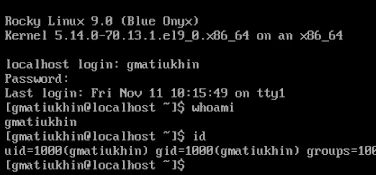
\includegraphics{1.png}\\
        \item Используя комманду \texttt{su} для переключения к учетной записи \verb!root!. При запросе пароля введите пароль пользователя \verb!root!.\\Объясните информацию комманды \verb!id!.
          \\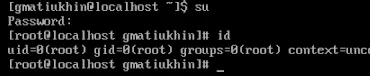
\includegraphics{2.png}\\
        \item Посмотрите в безопасном режиме файл \texttt{/etc/sudoers}
        \item Убедитесь, что в открытом файле присутствует строка\\ \texttt{wheel ALL=(ALL) ALL}\\
          \\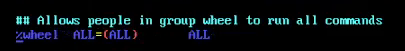
\includegraphics{3.png}\\
          Объясните, что это означает и для чего нужна группа \texttt{wheel}
        \item Создайте пользователя \texttt{alice}, входящего в группу \verb!wheel!
        \item Убедитесь, что пользователь \texttt{alice} добавлен в группу \verb!wheel!, введя \verb!id alice!
          \\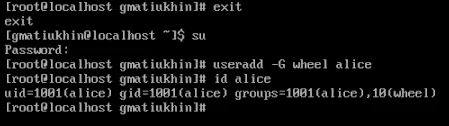
\includegraphics{4.png}\\
        \item Задайте пароль для пользователя \texttt{alice}
        \item Переключитесь на учетную запись пользователя \texttt{alice}
        \item Создайте пользователя \texttt{bob}
        \item Установите пароль для пользователя \texttt{bob}
          \\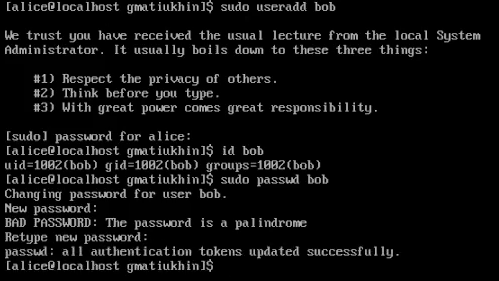
\includegraphics{5.png}\\
      \end{enumerate}
    \subsection{Создание учетных записей пользователей}
      Применим общие решения для создания учетных записей пользователей.
      \begin{enumerate}
        \item Перелючитесь в терминале на учетную запись пользователя \texttt{root}:
        \item Откройте файл конфигурации \texttt{/etc/login.defs} для редактирования.\\
          Убедитесь, что параметр \texttt{CREATE\_HOME} установлен в значение \texttt{yes}\\
          Установите параметр \texttt{USERGROUPS\_ENAB} в значение \texttt{no}
          \\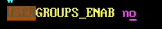
\includegraphics{6.png}
          \\\includegraphics{6\_1.png}
        \item Перейдите в каталог \texttt{/etc/skel/}, создайте каталоги \texttt{Pictures} и \texttt{Documents}
          \\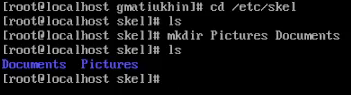
\includegraphics{7.png}\\
        \item Измените содержимое файла \texttt{~/.bashrc}, добавив строку:\\
          \texttt{export EDITOR=/usr/bin/vim}
          \\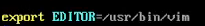
\includegraphics{8.png}\\
        \item Используя утилиту \texttt{useradd}, создайте пользователя \texttt{carol}
        \item Установите пароль для пользователя \texttt{carol}
        \item Посмотрите информацию о пользователе \texttt{carol}
          \\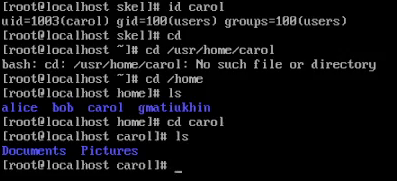
\includegraphics{9.png}\\
        \item Измените свойства пароля пользователя \texttt{carol} следующим образом
          \\
\includegraphics{10.png}\\
        \item Создайте еще несколько пользователей используя скрипт
          \\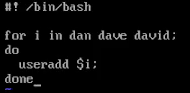
\includegraphics{11.png}\\
        \item Убедитесь, что идентификатор \texttt{alice} существует во всех трех файлах
        \item Убедитесь, что идентиыикатор \texttt{carol} существует не во всех трех файлах
          \\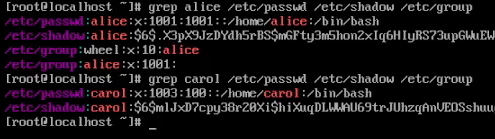
\includegraphics{12.png}\\
      \end{enumerate}
    \subsection{Работа с группами}
      В этом упражнении требуется создать две группы и добавить некоторых пользователей в эти группы
      \begin{enumerate}
        \item Находясь под учетной записью пользователя \texttt{root}, создайте группы \texttt{main} и \texttt{third}
        \item Используйте \texttt{usermod} для добавления пользователей \texttt{alice} и \texttt{bob} в группу \texttt{main}, а \texttt{carol}, \texttt{dan}, \texttt{dave} и \texttt{david} -- в группу \texttt{third}
          \\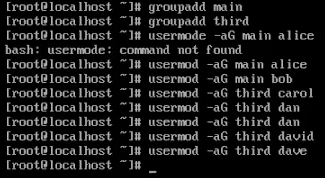
\includegraphics{13.png}\\
        \item Убедитесь, что пользователь \texttt{carol} правильно добавлен в группу \texttt{third}.\\
          Опредеделите, в какие вторичные группы входит \texttt{carol}.
          \\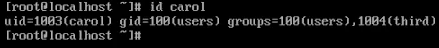
\includegraphics{14.png}\\
        \item Определите, участниками каких групп являются другие созданные вами пользователи
      \end{enumerate}
  \section{Контрольные вопросы}
    \begin{enumerate}
      \item При помощи какой команды можно получить информацию о номере, назначенном пользователю Linux, о группах, в которые включён пользователь?
        \\\texttt{id}
      \item Какой \texttt{UID} имеет пользователь \texttt{root}?
        \\0
      \item В чём состоит различие между командами \texttt{su} и \texttt{sudo}?
        \\И \texttt{su}, и \texttt{sudo} повышают привилегии, назначенные текущему пользователю. Основное различие между ними заключается в том, что для \texttt{su} требуется пароль целевой учетной записи, а для \texttt{sudo} требуется пароль текущего пользователя. Поэтому гораздо безопаснее использовать \texttt{sudo}, поскольку он не включает обмен конфиденциальной информацией.
      \item В каком конфигурационном файле определяются параметры \texttt{sudo}?
        \\\texttt{/etc/sudoers}
      \item Какую команду следует использовать для безопасного изменения конфигурации \texttt{sudo}?
        \\\texttt{visudo}
      \item Если вы хотите предоставить пользователю доступ ко всем командам администратора через \texttt{sudo}, членом какой группы он должен быть?
        \\\texttt{wheel}
      \item Какие файлы/каталоги можно использовать для определения параметров, которые будут использоваться при создании учётных записей пользователей?
        \\\texttt{/etc/login.defs}, \texttt{/etc/skel/*}
      \item В каких файлах хранятся пароли пользователей, учётные записи групп?
        \\\texttt{/etc/passwd}, \texttt{/etc/shadow}, \texttt{/etc/group}
      \item Какие команды вы можете использовать для изменения информации о пароле пользователя?
        \\\texttt{passwd}, \texttt{usermod}
      \item Сколько групп вы можете создать в файле \texttt{/etc/passwd}? Поясните свой ответ.
        \\В файле \texttt{/etc/passwd} нельзя создать группы, это можно сделать в файле \texttt{/etc/group}
      \item Какую команду следует использовать для изменения файла\\ \texttt{/etc/group} вручную?
        \\\texttt{visudo}
    \end{enumerate}
  \section{Вывод}
    В ходе выполнения данной работы я получил представление о работе с учётными записями пользователей и группами пользователей в операционной системе типа Linux
\end{document}
